\section{Experiment 2: HIGHLIGHTS-DIV}
Experiment 2 compared summaries generated by the HIGHLIGHTS-DIV algorithm with summaries generated by the basic HIGHLIGHTS algorithm and summaries generated by the \emph{Random} baseline (which significantly outperformed the \emph{First} baseline in Experiment 1). We recruited 48 participants through Amazon Mechanical Turk (25 female, Mean age = 36, STD = 11.6).  

\paragraph{Agent Selection Results} 
Figure~\ref{fig:highlightsDivRes} shows the correctness rates obtained by participants in experiment 2 for each of the summary methods. We begin by comparing HIGHLIGHTS summaries and HIGHLIGHTS-DIV summaries, which is the main focus of this experiment. 
%When analyzing participants' correctness rate for these summaries, we find an interaction effect between the summary method and comparison type, therefore fit a separate model for each comparison type. 
When making the high-difficulty comparison (\emph{200E} vs. \emph{400E} agents), participants were more likely to identify the superior agent when presented with HIGHLIGHTS-DIV summaries ($\chi^2=7.16, p=0.007, OR = 4.2$). We note that participants' performance when presented with HIGHLIGHTS summaries was lower than that of participants in Experiment 1 for the high-difficulty agent comparison. However, since we used a within-subject design, if participants were less attentive, they should also be less successful when presented with HIGHLIGHTS-DIV summaries. The difference between HIGHLIGHTS and HIGHLIGHTS-DIV remains significant even when aggregating the HIGHLIGHTS data from both experiments. We did not find  significant differences for the medium- and low-difficulty agent comparisons. 

When comparing the performance of participants when presented with \emph{Random} summaries with their performance when presented with HIGHLIGHTS or HIGHLIGHTS-DIV summaries, we did not observe an interaction effect between summary and comparison type. Therefore, we fit a single model for each summary comparison (\emph{Random} vs. HIGHLIGHTS and \emph{Random} vs. HIGHLIGHTS-DIV). We found a statistically significant effect for both comparisons, with participants being less successful when presented with \emph{Random} summaries (\emph{Random} vs. HIGHLIGHTS: $\chi^2=20.686, p<0.001, OR = 3.06$; \emph{Random} vs. HIGHLIGHTS-DIV: $\chi^2=27.28, p<0.001, OR = 5.15$). These results reinforce the results of Experiment 1 which showed improved performance with HIGHLIGHTS summaries compared to \emph{Random} summaries. Moreover, while in Experiment 1 we  found a significant difference only for the difficult agent comparison, here we observed significant differences for all agent comparisons.\footnote{It is reasonable to observe different performance levels with \emph{Random} summaries, as different participants could observe different \emph{Random} summaries.} When aggregating the data from both experiments for HIGHLIGHTS and \emph{Random}, we find significant differences for all agent comparisons, strengthening the conclusions from Experiment 1. 

The explanations given by participants for their agent choices were similar to those given by participants in Experiment 1. When making the high-difficulty comparison with the HIGHLIGHTS-DIV summaries, participants often referred to the fact that the summary of the \emph{200E} agent included a trajectory were Pacman was eaten, e.g. ``Player A [200E] gets caught by the ghosts at least once so it looks like Player B [400E] might have the better game'', or to the fact that the \emph{400E} agent was shown eating ghosts, e.g. ``Player B [400E] was able to eat some power pills and blue ghosts to gain more points.'' Explanations for the other comparisons were similar to those given when presented with HIGHLIGHTS summaries described in Section~\ref{sec:exp1res}.

\begin{figure}[h]
	%\centering
	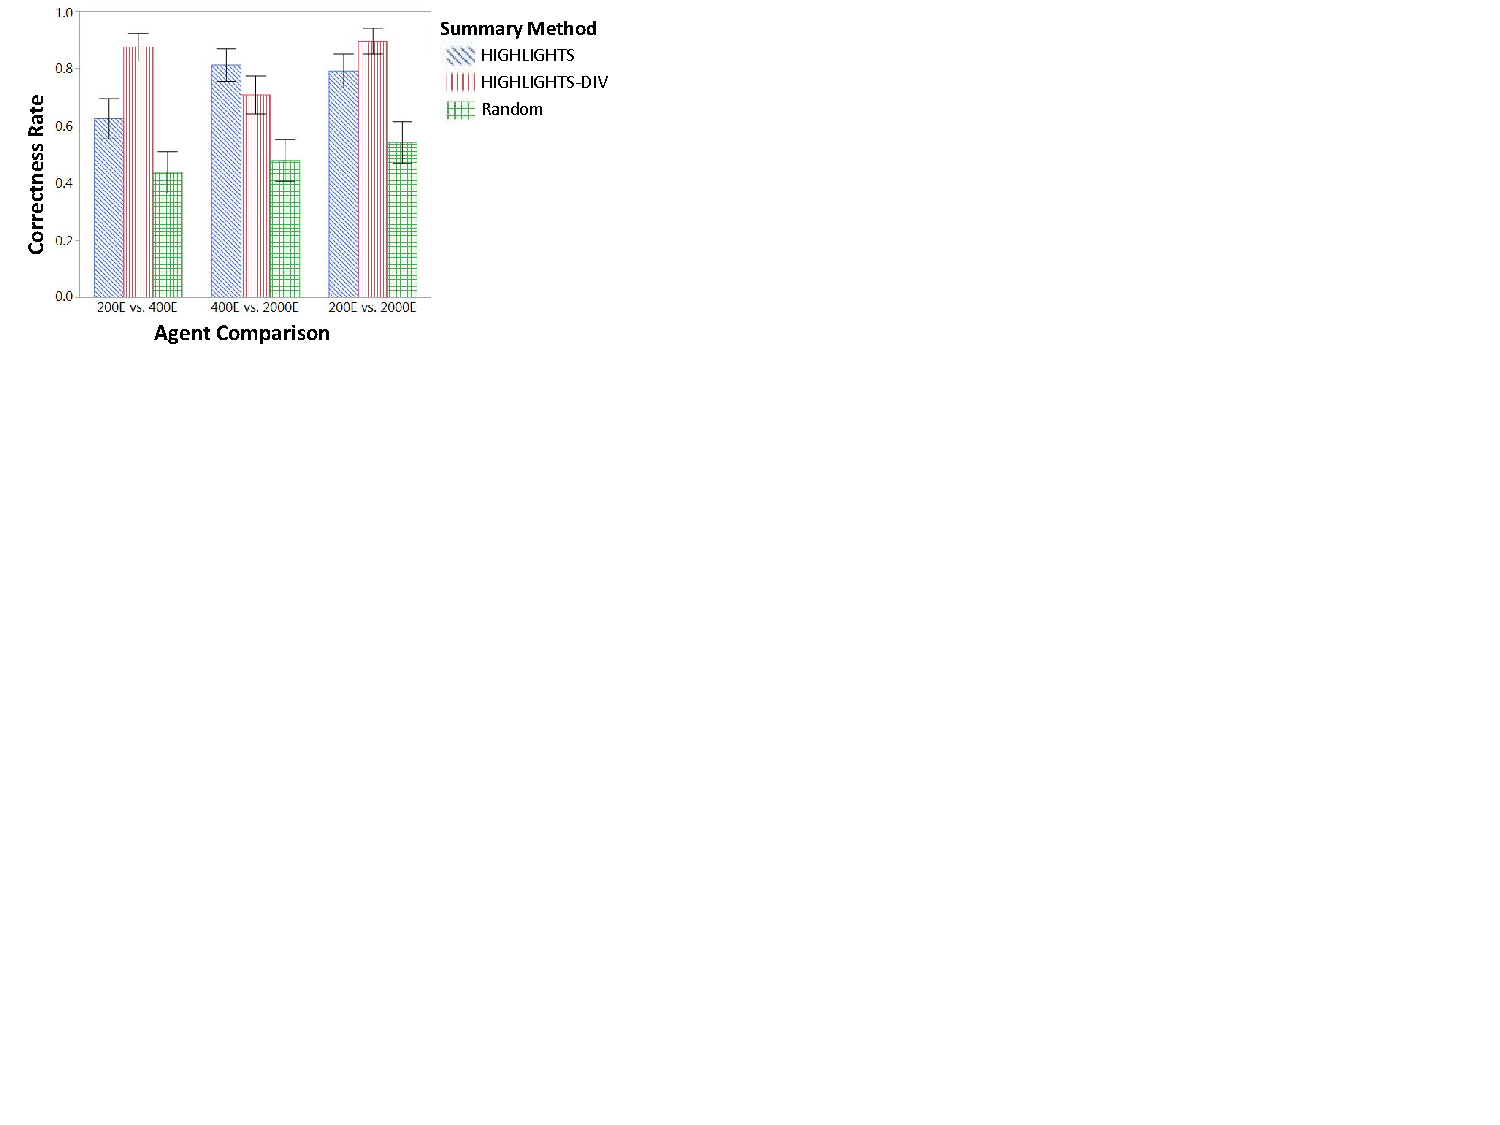
\includegraphics[width=0.9\columnwidth]{figs/correctnessExp2figForPaper.pdf}\\
	\caption{Correctness rate of participants in the agent selection task (Experiment 2).}
	\label{fig:highlightsDivRes}
	\vspace{-0.3cm}
\end{figure}

%The confidence ratings for all summary methods are shown in Figure~\ref{fig:highlightsConfExp2}. 
As in Experiment 1, we observed mixed results in terms of participants' confidence alignment with their actual performance. For the high-difficulty and low-difficulty agent comparisons, Participants' confidence ratings were significantly higher when presented with HIGHLIGHTS-DIV summaries compared to their confidence when reviewing HIGHLIGHTS summaries (high-difficulty: $\chi^2=17.84, p<0.001, OR = 3.68$; low-difficulty: $\chi^2=11.14, p=0.001, OR = 2.82$). We did not observe a statistically significant difference for the medium-difficulty comparison. The higher confidence when shown HIGHLIGHTS-DIV summaries is in line with participants' objective performance for the high-difficulty comparison. We did not find any differences in confidence ratings between HIGHLIGHTS and \emph{Random}, despite the significantly higher objective performance of participants when shown HIGHLIGHTS summaries. When comparing participants' confidence in the HIGHLIGHTS-DIV and \emph{Random} conditions, we found a statistically significant difference for the low-difficulty agent comparison ($\chi^2=16.24, p<0.001, OR = 3.72$). 


% \begin{figure}[h]
% 	%\centering
% 	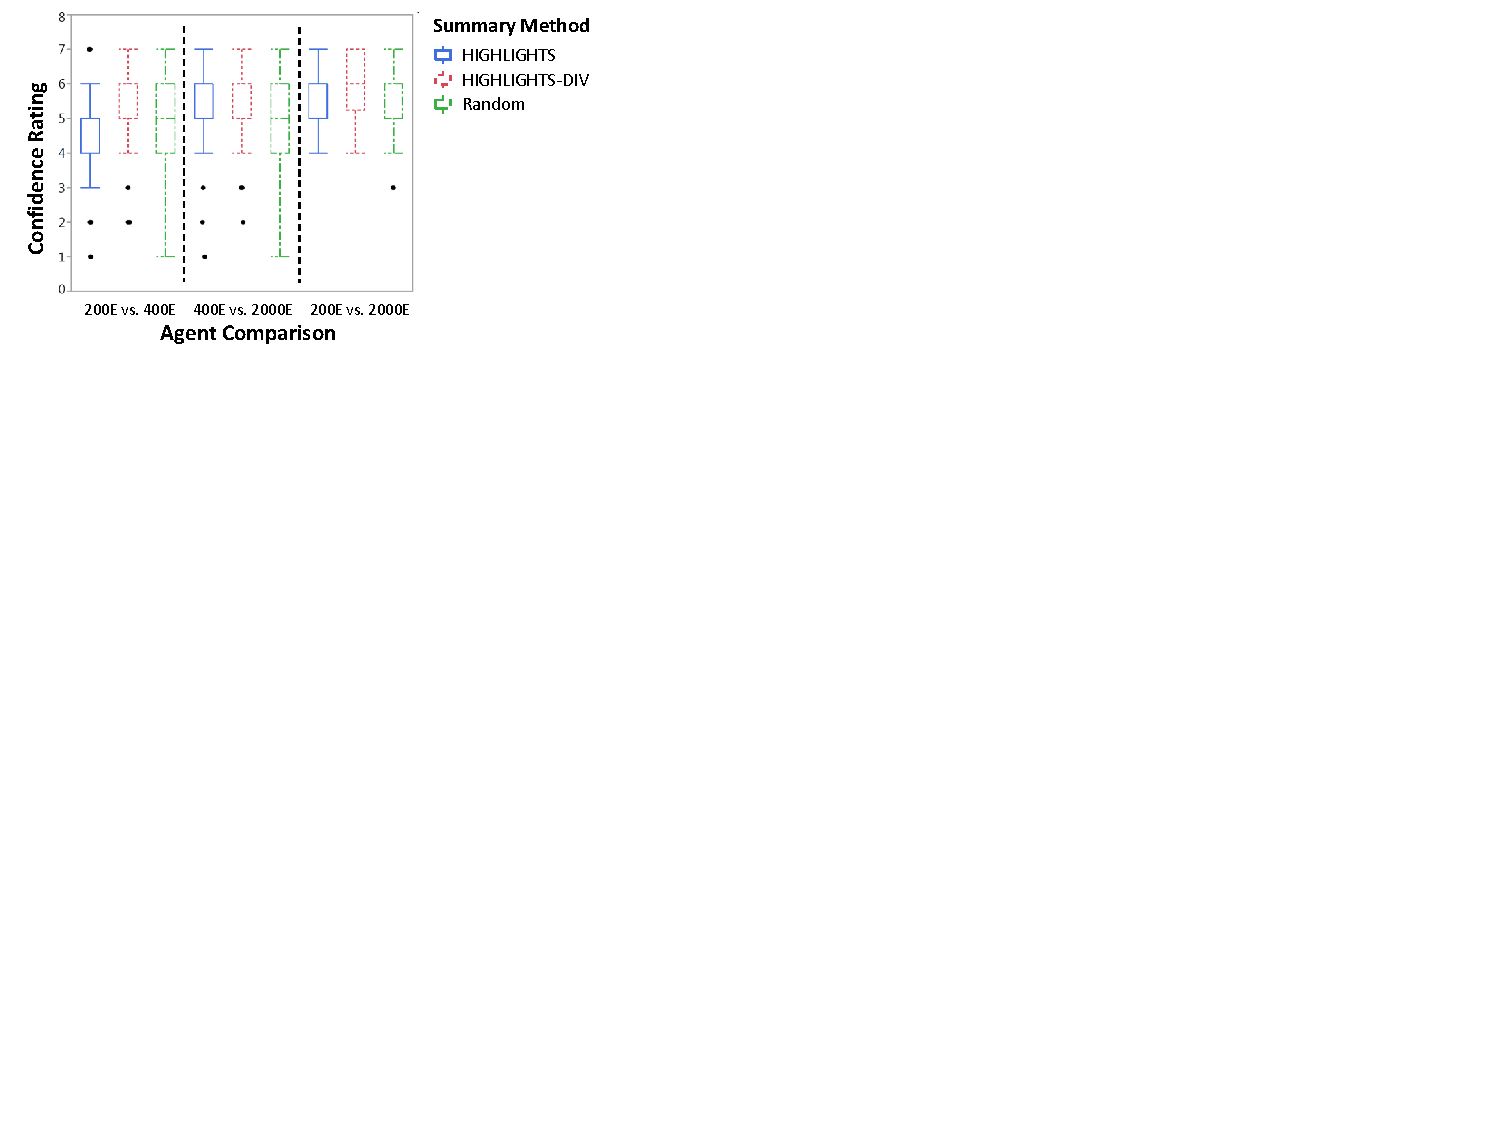
\includegraphics[width=0.85\columnwidth]{figs/confidenceExp2figForPaper.pdf}\\
% 	\caption{Participants' confidence rating on a scale of 1--7 when selecting an agent (Experiment 2).}
% 	\label{fig:highlightsConfExp2}
% 	\vspace{-0.4cm}
% \end{figure}


\paragraph{Summary Preferences}
%Figure~\ref{fig:highlightsPrefsExp2} shows the distribution of participants' preferences ratings.
%\footnote{In Experiment 2 we did not elicit preferences for the \emph{200E} agent summaries to obtain more data for the \emph{400E} and \emph{2000E} agents, for which there were greater differences between different summaries.}
When presented with summaries of the \emph{400E} agent, participants preferred the HIGHLIGHTS-DIV summary over the HIGHLIGHTS summary, though this preference was only marginally significant ($Median = 3, p=0.1$). When explaining their ratings of these summaries participants often referred to skills demonstrated in the summary, e.g. ``The types of explanations provided were similar to those given in Experiment 1 and often referred to the skills demonstrated in the summary, e.g. ``It [HIGLIGHTS-DIV] shows how well the player baited the ghosts and then was able to snack on them.'' We found no difference in preferences between the two summary methods when reviewing summaries of the \emph{2000E} agent  ($Median = 4$). When comparing participants' preferences for HIGHLIGHTS and \emph{Random} summaries, we observed similar results to those obtained in Experiment 1 ($Median = 5$). As in Experiment 1, the difference was significant only when comparing summaries of the \emph{2000E} agent ($Median = 5, p = 0.05$). We did not directly compare HIGHLIGHTS-DIV with \emph{Random} summaries, but the results suggest a preference for HIGHLIGHTS-DIV summaries (as they were preferred over HIGHLIGHTS summaries, which were preferred over \emph{Random} summaries).  
%Participants subjective preferences ratings for summary are shown in Figure~\ref{fig:highlightsPrefs}. Recall, that a rating closer to 7 is means they stated that the summary generated by HIGHLIGHTS was more helpful in assessing the agent's capability, while a rating closer to 1 indicates that they found the other summary (either generated by either \emph{First} or \emph{Random} as more helpful). That is, ratings greater than 4 indicate a preference for HIGHLIGHTS. The ratings are shown separately for each type of agent for which summaries were presented. 

% \begin{figure}[h]
% 	%\centering
% 	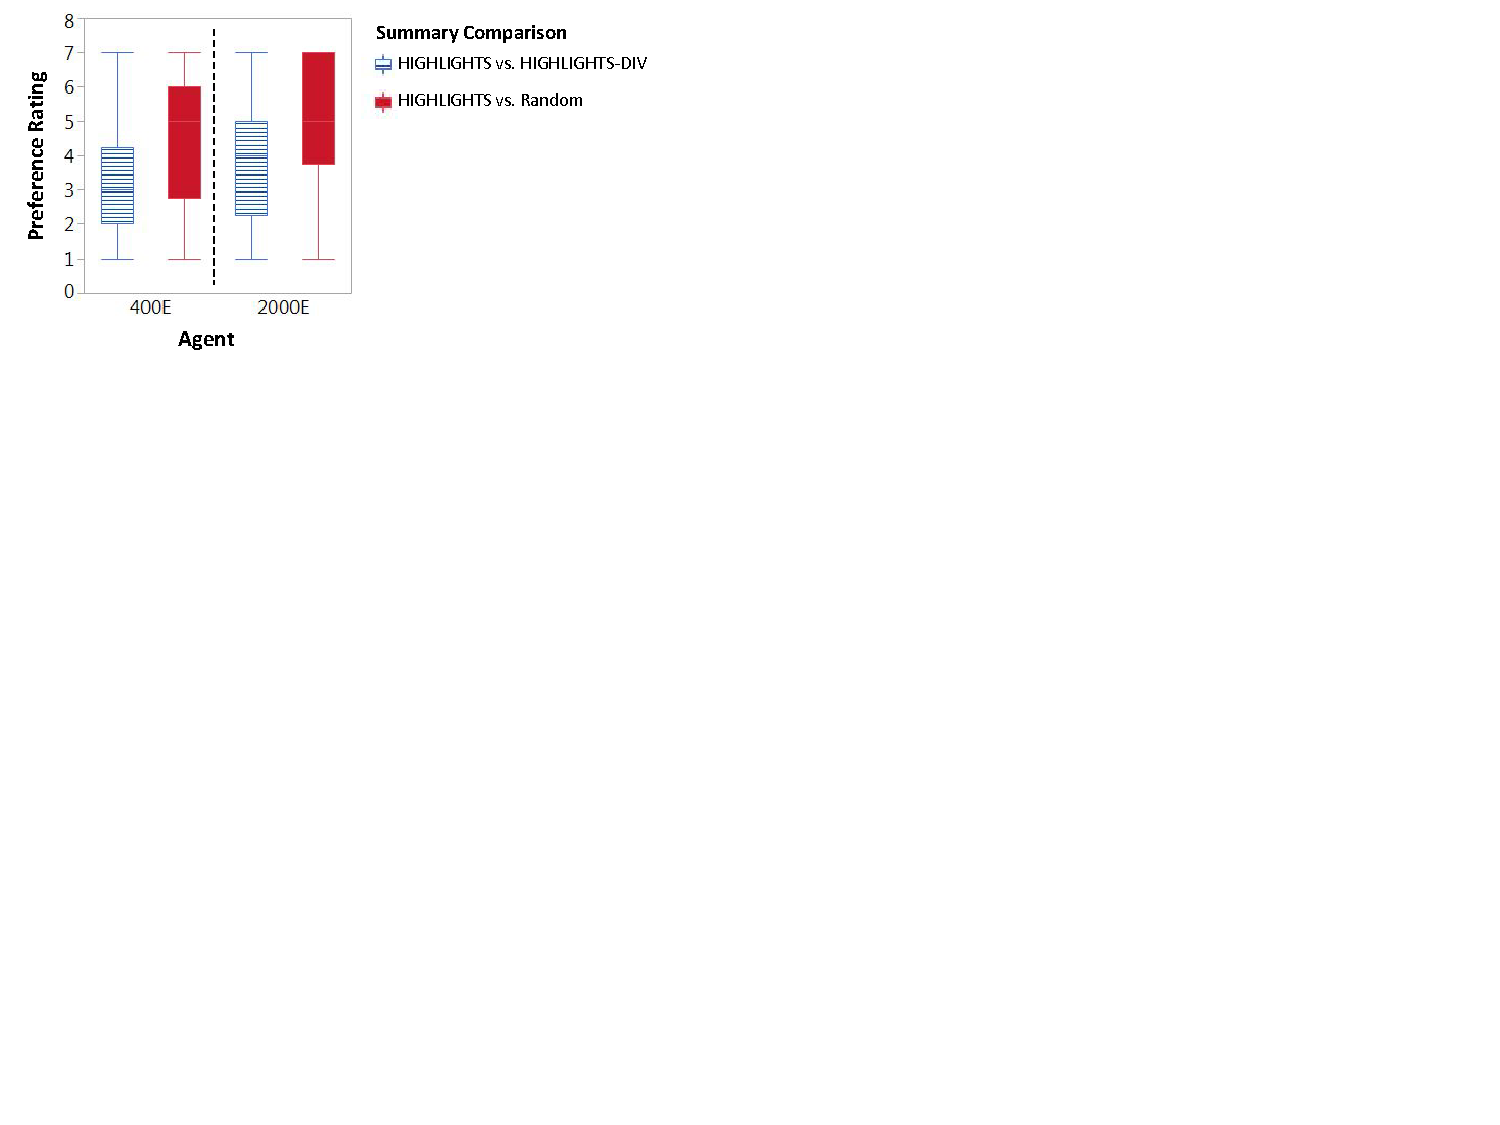
\includegraphics[width=0.8\columnwidth]{figs/preferencesExp2figForPaper.pdf}\\
% 	\caption{Participants' preference rating on a scale of 1--7, where 7 = ``HIGHLIGHTS is more helpful'' (Experiment 2).}
% 	\label{fig:highlightsPrefsExp2}
% 	\vspace{-0.3cm}
% \end{figure}

%On average, participants preferred summaries generated by HIGHLIGHTS over summaries generated by \emph{First} ($Median = 6$) and compared to summaries generated by \emph{Random} ($Median = 5$). The only statistically significant differences were in preferences for HIGHLIGHTS summaries were for the highest performing agent (the ``2000'' agent). The ratings were significantly greater than 4 both when comparing HIGHLIGHTS with \emph{First} ($Median = 7, p<0.001$) and when comparing HIGHLIGHTS with \emph{Random} ($Median = 6, p=0.009$). We attribute this stronger preference to the greater difference between summaries generated by different methods when considering agents that have more capabilities. For example, the highest performing Pacman agent was able to both escape ghosts and eat the power pills which let it eat ghosts. The HIGHLIGHTS summary for this agent included trajectories demonstrating this capability, while \emph{First} summaries did not show it, and only some \emph{Random} summaries did (by chance). This made for a meaningful difference between the summaries. In contrast, the lowest performing agent did not have many capabilities, and therefore there was less difference between the summaries generated by the different methods. 


